\section{Subsystem Decomposition}
The \texttt{DriveIT System} can be split into five main subsystems - the \texttt{DriveIT Windows Client}, \texttt{CarQuery}, \texttt{DriveIT Web Client}, \texttt{DriveIT Web API}, and \texttt{Persistent Storage} subsystems. 
These subsystems are described below. 

\subsection{The DriveIT System}
\begin{figure}[H]
	\centering
	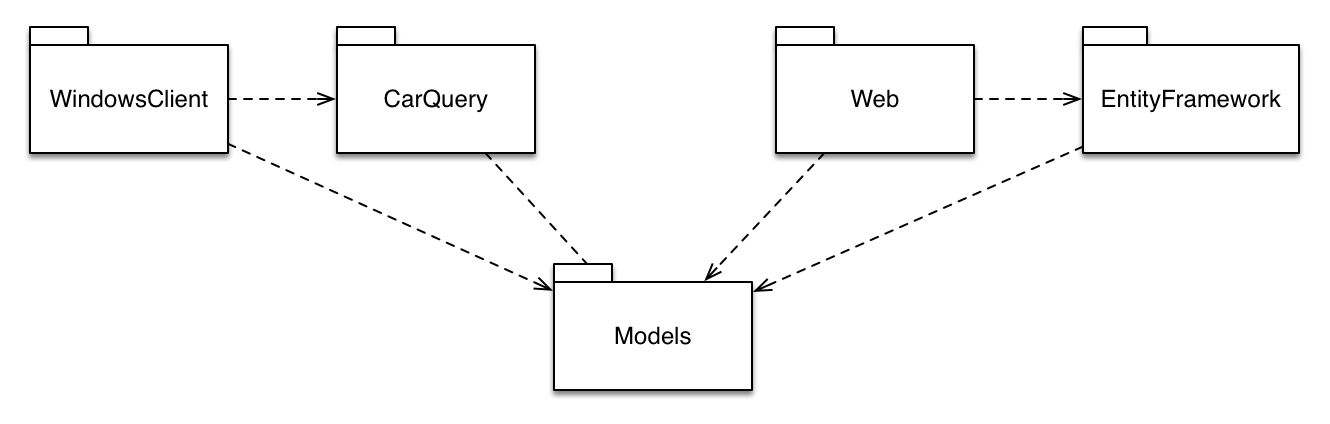
\includegraphics[width=\textwidth]{Figures/DriveITSubsystemDecomposition}\\
	\caption{Subsystems of the \texttt{DriveIT System}.}
\end{figure}

\subsection{Persistent Storage Subsystem} 
The Persistent Storage Subsystem manages storing and retrieving entity objects using the \textit{Entity Framework} and its serialisation functionality.\\
The serialised entities are stored in a \textit{Microsoft SQL Database} which is hosted on \textit{Microsoft Azure}. The subsystem provides the \texttt{DriveIT Web API} with deserialised entities, which uses the entities to provide the backend for other subsystems.\\
The subsystem supports retrieving all Entities of a given type, a specific entity using its unique ID, and retrieving an entity on its relation to other entities.
The Persistent Storage Subsystem consists of two classes and an interface (see figure \ref{fig:entityframeworksubsystem}). \texttt{EntityStorage} is the repository working on top of the \textit{Entity Framework} database layer, \texttt{DriveITContext}, providing the \texttt{IPersistentStorage} interface.

\begin{figure}[H]
	\centering
	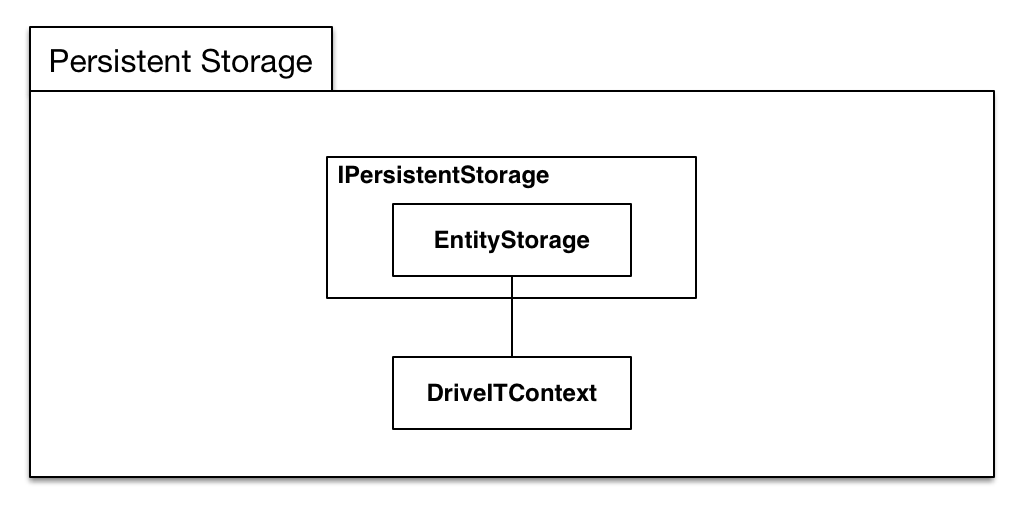
\includegraphics[width=\textwidth]{Figures/EntityFrameworkSubsystemDecomposition}
	\caption{Classes in the Persistent Storage Subsystem.}
	\label{fig:entityframeworksubsystem}
\end{figure}

\subsection{Web API}
The \texttt{DriveIT Web API}, which is built on \textit{ASP.NET Web API}\footnote{\url{http://www.asp.net/web-api}}, provides public communication with the \texttt{Persistent Storage} subsystem. This is done using specific URL routes. Furthermore it enforces authorisation so unauthorized users, and users with different user roles, only have limited access to the data of the \texttt{DriveIT System}.\\ 
Every table in the \texttt{Persistent Storage} subsystem must therefore be supported by the web API, although not every table is available to every user.\\
The \texttt{DriveIT Web API} is comprised of a series of modules for serialising the Model Entities into \texttt{JSON}\footnote{\url{http://en.wikipedia.org/wiki/JSON}} or \texttt{XML}\footnote{\url{http://en.wikipedia.org/wiki/XML}} and transferring these via a \texttt{REST} interface accessible using \texttt{HTTP}.\\
These modules are built into \textit{ASP.NET Web API}, and are not handled in our code.\\

The Web API consists of several controllers which uses a static class to translate \texttt{DTO's}\footnote{\url{http://en.wikipedia.org/wiki/Data_transfer_object}} into entities and vice versa. It is also the controllers that check for special cases, e.g. when a customer wants to update or delete a comment, and it is not allowed to change other \texttt{Customer}s' comments.

\subsection{Windows Client} 
\begin{figure}[H]
	\centering
	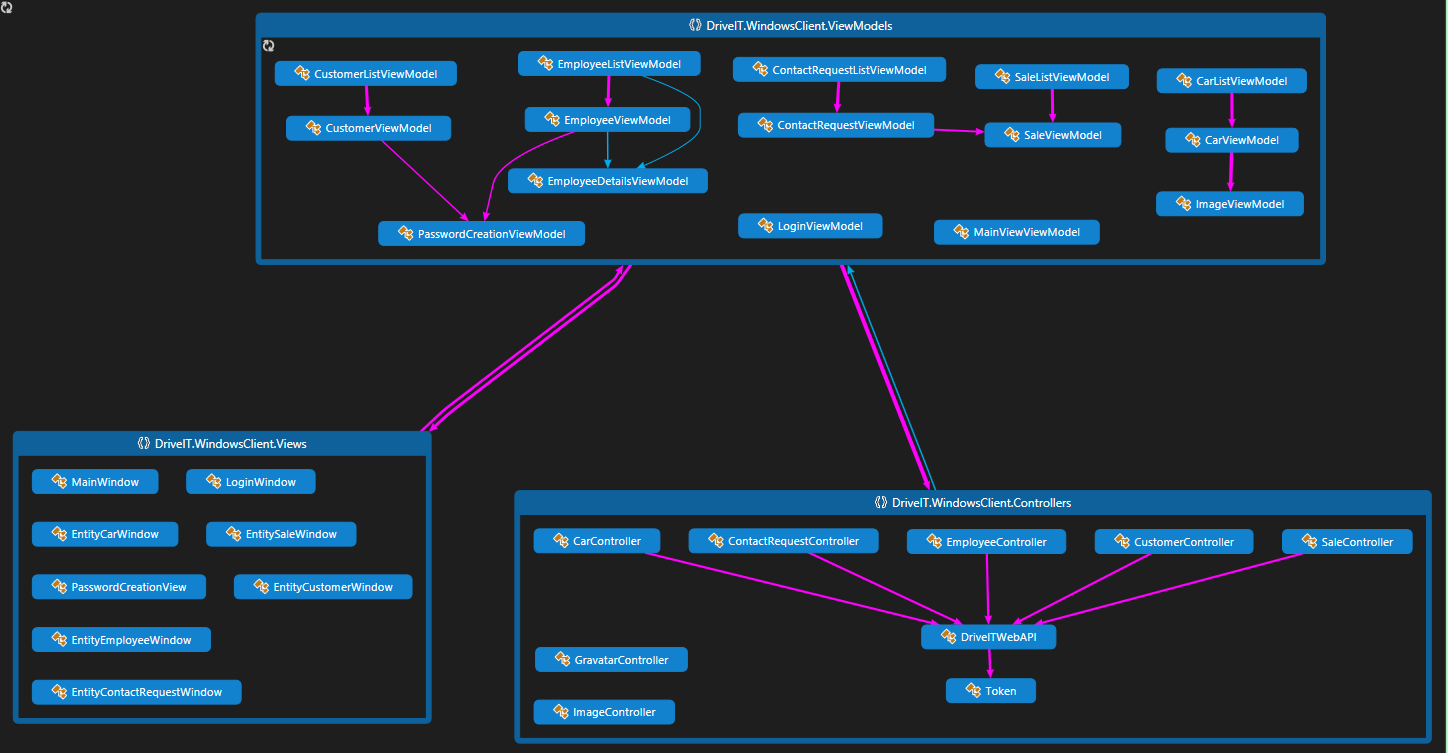
\includegraphics[width=\textwidth]{Figures/WindowsClientCodeMap}
	\caption{The Code Map of the Windows Client}
	\label{fig:WindowsClientCodeMap}
\end{figure}
The Windows Client is used by the \texttt{Employee}s, to manipulate data in the system. Depending on their role, \texttt{Employee} or \texttt{Administrator}, they can \textit{CRUD} all entities except for creating \texttt{ContactRequest}s.\\

The \texttt{Employee} signs in to the client with his or her email and password, and can then use the user interface to manipulate data in the \texttt{DriveIT System}.\\
The subsystem is made out of three main components: The \texttt{Views}, the \texttt{ViewModels} and the \texttt{Controllers}.\\
The \texttt{Views} package contains the user interface written in Windows Presentation Foundation (henceforth WPF). The \texttt{ViewModels} package contains the \texttt{ViewModel}s which hold data bound to the \texttt{View}s following Microsoft's \textit{Model View ViewModel} architectural pattern\footnote{\url{http://en.wikipedia.org/wiki/Model_View_ViewModel}}.

\texttt{ViewModel}s for entities are often created in the form of a \texttt{EntityListViewModel} and a \texttt{EntityViewModel}, but a few extra \texttt{ViewModel}s exists for additional \texttt{Views}s such as the \texttt{LoginViewModel} and the \texttt{PasswordCreationViewModel}.

The \texttt{Controllers} package contains the \texttt{Controller}s which transforms data and sends and receives HTTP requests to and from the \texttt{DriveIT Web API}. Images are uploaded to \textit{Azure Blob Storage}. To provide \texttt{Employee}s and \texttt{Customer}s with profile pictures, a \texttt{GravatarController} exists to convert email strings into \textit{Gravatar}\footnote{\url{https://en.gravatar.com/}} profile URLs.

\subsection{Web Client}
The \texttt{DriveIT Web Client} is accessable through the internet, whereas it is being used by non-registered users and customers, who already have registered themselves through the web client and logged on. The web client is being used to search for cars, that are being sold by the company using the \texttt{DriveIT System}, CRUD comments (if the customer is logged in, else it's only read), CRD contact requests, read orders and read employees (contact tab). A customer is also able to create, read and update information regarding their own user account.\\
The web client is based on the ASP.NET MVC framework, that is implementing the MVC design pattern. The subsystem is made of three components: Models, Views and Controllers. The views contains the user interface and is written in cshtml, which is a mix of C$\sharp$ and HTML code. The models contains lists of database records and the controllers are responsible for giving the models, filled with database records, to the views, for them to display the data in the model.

\subsection{CarQuery} 
This subsystem is a collection of classes that enable the rest of the \texttt{DriveIT System} to fill out missing information about cars from the CarQuery API.\\
The sub system is used by an employee when creating a new car. The subsystem mainly consists of a \texttt{JSON} deserialiser that communicates with the \texttt{CarQuery REST API} and another class that receives a Car object and fills out the missing attributes using the deserialised JSON data. \\
The employee fills out the information he/she knows about the car and the system then narrows its information search against the \texttt{CarQuery REST API}.
\begin{figure}[H]
	\centering
	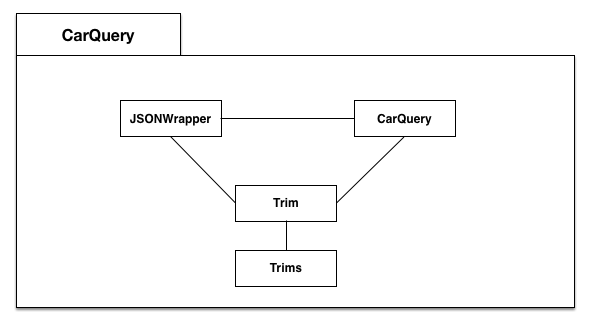
\includegraphics[width=\textwidth]{Figures/CarQuerySubsystemDecomposition}\\
	\caption{Subsystems of the CarQuery Subsystem.}
\end{figure}